\documentclass{amsart}
\usepackage{graphicx}
\graphicspath{{./}}
\usepackage{hyperref}
\usepackage{csvsimple}
\usepackage{longtable}
\usepackage{lscape}
\usepackage{epigraph}
\title{The Hidden Trust Profile of the Human Race}
\author{Zulfikar Moinuddin Ahmed}
\date{\today}
\begin{document}
\maketitle

\section{What is the Trust Profile of the Human Race?}

We have succeeded in producing a smoothly varying set of Barndorff-Nielsen (Generalised Hyperbolic) densities that represent the trust characteristics of the Human Race along with a natural distance metric for closeness.

What allows this possibility is the overdetermined nature of the five parameters of GHD with various optimisations.  We now have relatively good estimates to calibrate the deformation profile from Trust in Family to Trust in people of Other Nationalities.

Our next order of business is to study in more fine detail regions of trust in closer and more distant relative positions.  For example, what is the profile {\em closer than Family?} or closer to Family than people known to us.  The shape contains the full spectrum of trust levels from complete trust to complete distrust.

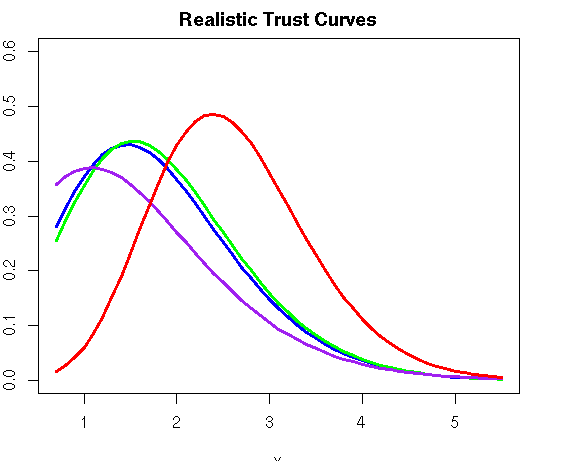
\includegraphics[scale=0.8]{trust_curves.png}

The blue is family, and red is an unknown stranger.  Purple is intimate relationship.

These are realistic calibrated curves and give direct probability.

\begin{verbatim}
# Use Other to determine the trust
# densities of the human race
ab <- c( 0.010585097,  0.019156924, -0.006620259, 0.007031738,
         0.011095266,  1.943972143, -2.919369783, -0.247401488,
         0.518246653,  1.363879411)

tref <- c( 0, 35.30684, 42.12769, 287.43995,  53.64879)

# Inference 0-35.3 is closer than neighbor or known
# person

g<-function( theta ){
  lambda<-theta[1]
  mu <- theta[2]
  sigma <- theta[3]
  gamma <- theta[4]
  alpha.bar <- theta[5]
  out <- ghyp( lambda=lambda,mu=mu,sigma=sigma,
               gamma=gamma,alpha.bar=alpha.bar)
  out
}

trust_theta<-function( t ){
  tau<-rep(0,5)
  a<-ab[1:5]
  b<-ab[6:10]
  for (r in 1:5){
    tau[r] <- b[r] + a[r]*t
  }
  theta <- exp( tau )
  theta  
}

trust_curve<-function( x, t ){
  theta <- trust_theta( t )
  dghyp(x, object=g(theta) )
}
\end{verbatim}

\end{document}

